\documentclass[xcolor=x11names,compress,professionalfonts]{beamer}

%% General packages %%%%%%%%%%%%%%%%%%%%%%%%%%%%%%%%%%
\usepackage[utf8]{inputenc}
\usepackage{graphicx}
\usepackage{tikz}
\tikzset{% change default arrow tips
    >=latex
}
\usepackage{ifthen}

\usepackage{amsmath}
\usepackage{nicefrac}

\usepackage{color}

%%%%%%%%%%%%%%%%%%%%%%%%%%%%%%%%%%%%%%%%%%%%%%%%%%%%%%


%% Beamer Layout %%%%%%%%%%%%%%%%%%%%%%%%%%%%%%%%%%
\useoutertheme[subsection=false,shadow]{miniframes}
\useinnertheme{rectangles}

\setbeamertemplate{navigation symbols}{}%remove navigation symbols

\newcommand{\btVFill}{\vskip0pt plus 1filll}%place an element at the bottom of the page

\usepackage{libertine}
\usepackage[T1]{fontenc}

\setbeamerfont{title like}{shape=\scshape}
\setbeamerfont{frametitle}{shape=\scshape}

\setbeamercolor*{lower separation line head}{bg=DeepSkyBlue4} 
\setbeamercolor*{normal text}{fg=black,bg=white} 
\setbeamercolor*{alerted text}{fg=red} 
\setbeamercolor*{example text}{fg=black} 
\setbeamercolor*{structure}{fg=black} 
 
\setbeamercolor*{palette tertiary}{fg=black,bg=black!10} 
\setbeamercolor*{palette quaternary}{fg=black,bg=black!10} 

\renewcommand{\(}{\begin{columns}}
\renewcommand{\)}{\end{columns}}
\newcommand{\<}[1]{\begin{column}{#1}}
\renewcommand{\>}{\end{column}}

\definecolor{BostonBlue}{HTML}{00688B}
\definecolor{Complementary}{HTML}{8B2300}
%%%%%%%%%%%%%%%%%%%%%%%%%%%%%%%%%%%%%%%%%%%%%%%%%%

\usepackage{braket}
% compile child documents using this preamble
\usepackage{subfiles}

%%%My Math

\newcommand{\pd}[2]{\frac{\displaystyle \partial #1}{\displaystyle\partial #2}} % for partial derivatives
\newcommand{\dx}{\mathrm{d}x}
\renewcommand{\d}[1]{\mathrm{d}#1}
\newcommand{\nth}{$n^\text{th}$ }

\newcommand{\mean}[1]{\langle #1 \rangle}
\DeclareMathOperator{\Pf}{Pf}
\DeclareMathOperator{\Tr}{Tr}

% idos
\newcommand{\id}{\ensuremath{\text{idos}}}
% mean energy of a gap
\newcommand{\me}{\ensuremath{\langle E \rangle}}
\newcommand{\mep}{\ensuremath{\langle E' \rangle}}
% bold g letter in math mode
\newcommand{\gv}{\ensuremath{\mathbf{g}}}
% the symbol used for the Fibonacci substitution matrix
\newcommand{\sub}{\ensuremath{M}}


\begin{document}


\begin{frame}
\title{{\fontsize{14}{60}\selectfont Gap structure of 1D cut and project Hamiltonians}}

\author{Nicolas Macé, Anuradha Jagannathan, Frédéric Piéchon}

\institute % (optional)
{
  Laboratoire de Physique des Solides\\
  Université Paris-Saclay
}

\date{September 20, 2016}

\titlepage

\btVFill
\begin{columns}
\begin{column}{2cm}
~\\
~\\
~\\
~\\
\raggedright
\includegraphics[scale=.15]{img/LogoUPSUD.png}
\end{column}
\begin{column}{6cm}
\centering
\includegraphics[width=1.\textwidth]{img/cover_illustration.pdf}
\end{column}
\begin{column}{2cm}
~\\
~\\
~\\
~\\
\raggedleft
\includegraphics[scale=.15]{img/logo-lps.jpg}
\end{column}
\end{columns}
\end{frame}

\begin{frame}
\frametitle{Outline}
\tableofcontents[hideallsubsections]
\end{frame}

\section{The gap labeling theorem}
%Each section needs a subsection for the small points on top to show up
\subsection{Dummy}

\begin{frame}{Electrons on quasiperiodic chains}
\begin{columns}
\begin{column}{8.5cm}
	\centering
	\includegraphics[scale=.7]{img/cut_and_project.pdf}
\end{column}

\begin{column}{3cm}
Approximants:
\begin{align*}
\alpha_l &= \frac{p_l}{q_l} \\
\alpha_l &\rightarrow \alpha
\end{align*}
\end{column}
\end{columns}

	$
		\text{Hamiltonian: } H(\alpha) = \sum_{x \in \mathbf{Z}} t_{x,x+1} \ket{x} \bra{x+1} + \text{h.c.}
	$
	
	2 lengths $\to$ 2 jump amplitudes $t_{x,x+1} = t_{1}$ or $t_2$.	
\end{frame}

\begin{frame}{The electronic spectrum}

A convenient way to plot the spectrum: the integrated density of states ($\id$).

$\id(E) = $ fraction of states below energy $E$

{\centering
\includegraphics[scale=.35]{img/idos_scaling.pdf}

\small{\id~of the Fibonacci Hamiltonian}

}

\begin{itemize}
	\item Electronic spectrum of quasiperiodic chains is hard to describe
	\item Rather: describe the $\id$ in the gaps $\to$ \textbf{gap labeling theorem}
\end{itemize}
\[
	\id(E\in \text{gap}) = n \tau^{-2} \mod 1
\]

\end{frame}

\begin{frame}{The gap labeling theorem}
The IDOS inside spectral gaps can be indexed using the irrational involved in the construction of the chain
	\[
		\id(E \in \text{gap}) = \frac{n}{1+\alpha} \mod 1
	\]
\begin{itemize}
	\item Constrains the spectrum... but is not enough to reconstruct it
	\item Model independent! (while the spectrum is model dependent) $\to$ a topological invariant
\end{itemize}

TODO: plot the idos for the diagonal and the on-site potential models

\end{frame}

\begin{frame}{The gap labeling theorem}
\[
		\id(E \in \text{gap}) = \frac{n}{1+\alpha} \mod 1
	\]
\begin{itemize}
	\item Has the gap label $n$ a physical interpretation?
\end{itemize}
\begin{itemize}
	\item Can the theorem be applied to approximants? 
	\item Does it help understanding the quasiperiodic limit?
\end{itemize}

\end{frame}

\begin{frame}{A simple, but incorrect proof}
Let $\alpha_l = \frac{p_l}{q_l} \to \alpha$ be a sequence of approximants.

$N_l = p_l + q_l$ is the maximum number of energy bands.

\[
	\id(E \in \text{gap}) = \frac{j(E)}{N_l}
\]
We can find integers $n$, $k$ such that $j = n q_l + k N_l$.
\[
	\id(E \in \text{gap}) = \frac{n q_l}{p_l + q_l} \mod 1
\]
Letting $l \to \infty$,
	\[
		\id(E \in \text{gap}) = \frac{n}{1+\alpha} \mod 1
	\]

\only<1>{
}
    
\only<2>{
	\begin{alertblock}{Problem}
$n$ may depend on $l$.
\end{alertblock}
}

\end{frame}

\section{The Fibonacci chain}
\subsection{Dummy}

\begin{frame}{A concrete example}
Gaps of successive approximants of the Fibonacci chain.

{\centering
\includegraphics[scale=.6]{img/gap_labels.pdf}

}
Call $\me_l$ the mean energy of a gap, and $\Delta_l(\me)$ its width. 
I identify two gaps if they overlap:
\[
	0.5 \Delta_l(\me) > |\me_l - \mep_{l+1}|
\]
\end{frame}


\begin{frame}{Stable and transient gaps}
{\centering
\includegraphics[scale=.65]{img/gap_labels.pdf}

}
%We identify a gap by its mean energy $\me$.
\begin{itemize}
	\item {\color{Complementary}Red labeled} gaps closes as $l \to \infty$ $\to$ {\color{Complementary}transient} gaps.
	\item {\color{BostonBlue}Blue labeled} gaps stay open $\to$ {\color{BostonBlue}stable} gaps.
\end{itemize}

\end{frame}

\begin{frame}{Stable and transient gaps}
{\centering
\includegraphics[scale=.6]{img/gap_labels.pdf}

}

\begin{itemize}
	\item {\color{BostonBlue}Blue gaps} have a well-defined label. The naive proof works!
	\item {\color{Complementary}Red gaps} have an ill-defined label but disappear.
\end{itemize}
$\to$ the naive proof works and correctly labels the gaps.
\end{frame}

\begin{frame}{Recursive gap labeling}

\begin{columns}
\newcommand{\s}{.2}

  \begin{column}{5cm}
  Recursive construction of the spectrum...
  \centering
     \includegraphics[scale=.35]{img/recursive_construction_spectrum.pdf}
  \end{column}


  \begin{column}{5cm}
  ...translates into recursive construction of the gaps!
  
		\begin{align*}
			G_{l}^{\text{left}} &= \sub^{-2} G_{l-2} \\
			G_{l}^0 &= \sub^{-3} G_{l-3} + \gv_1 \\
			G_{l}^\text{right} &= \sub^{-2} G_{l-2} + \gv_2
		\end{align*}

Where $G_l$ is the set of labels:

$\small{G_l = \{(m,n)| \id = n/(1+\alpha) + m\}}$

\[
			\sub = \begin{bmatrix}
				1 & 1\\
				1 & 0\\
			\end{bmatrix}
			\]
  \end{column}

\end{columns}


\begin{itemize}
	\item {\color{BostonBlue}Stable gaps} are the iterates of the 2 main gaps
	\item {\color{Complementary}Transient gaps} are the iterates of the central gap.
\end{itemize}

\end{frame}

\section{General case}
\subsection{Dummy}
\begin{frame}{General case}
We plot the gapwidth $\Delta_l$ as a function of the label for various quasiperiodic chains:

{\centering
\newcommand{\s}{.45}
\includegraphics[scale=\s]{img/loggapwidth_fibonacci_l_17.pdf}\\
\includegraphics[scale=\s]{img/loggapwidth_sqrt3_l_12.pdf}

}
\begin{itemize}
	\item The width decreases as a power-law of the label
	\item Above a critical label, all gaps are transient
	\item Recursive gap labeling using the Hofstadter rules?  \small{[Rüdinger, Piéchon 98]}
\end{itemize}

	
\end{frame}

\section{Conclusion}
\subsection{Dummy}
\begin{frame}{Conclusion and perspectives}
\begin{itemize}
	\item The gap labeling theorem can be extended to approximants
	\item The price to pay is the introduction of transient gaps, absent in the quasiperiodic case
	\item Gap labels have a physical meaning:
	\begin{itemize}
		\item It orders gap by decreasing width
		\item It separates stable from transient gaps
		\item It can be interpreted as a Chern number \small{[Levy \emph{et al} 2015]}
	\end{itemize}
\end{itemize}
Perspectives:
\begin{itemize}
	\item Understand the gap width behavior with the gap label
	\item Investigate to 2D quasicrystals, which also have gaps \small{[Prunelé \emph{et al} 2002]}
\end{itemize}
\end{frame}

\end{document}
